\documentclass[tikz]{standalone}
\usepackage{ctex}
\begin{document}
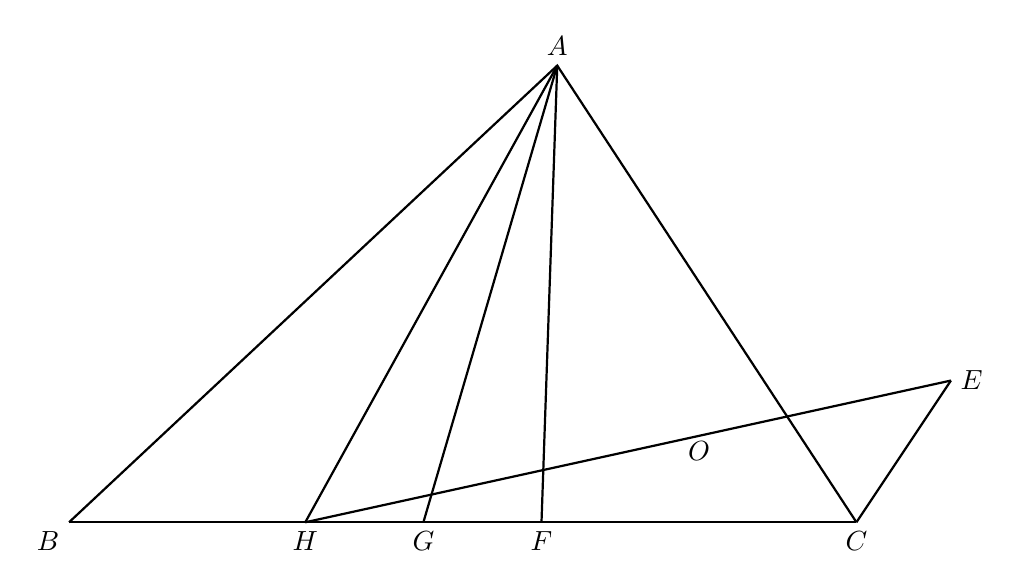
\begin{tikzpicture}[scale=1]
  % Points
  \coordinate (B) at (0,0);
  \coordinate (D) at (3,0);
  \coordinate (G) at (4.5,0);
  \coordinate (F) at (6,0);
  \coordinate (C) at (10,0);
  \coordinate (A) at (6.2,5.8);
  \coordinate (E) at (11.2,1.8);

  % Segments
  \draw[thick] (B) -- (C);
  \draw[thick] (B) -- (A) -- (C);
  \draw[thick] (D) -- (A);
  \draw[thick] (G) -- (A);
  \draw[thick] (F) -- (A);
  \draw[thick] (D) -- (E);
  \draw[thick] (C) -- (E);

  % Labels
  \node[above] at (A) {$A$};
  \node[below left] at (B) {$B$};
  \node[below] at (D) {$H$};
  \node[below] at (G) {$G$};
  \node[below] at (F) {$F$};
  \node[below] at (C) {$C$};
  \node[right] at (E) {$E$};
  \node at (8.0,0.9) {$O$};
\end{tikzpicture}
\end{document}
